\chapter{序論} \label{chap:jyoron}


\section{研究背景}%\label{sec:background}

前世紀の初めにロンドンのマンチエスター・スクエーアで，走り廻ったり，球をころがして遊んだり，おりおり妹に気をつけたりしていた子供があった．すぐ側のヤコブス・ウエルス・ミュースに住んでいて，学校通いをしていた子供なのだ．
通りがかりの人で，この児に気づいた者は無論たくさんあったであろうが，しかし誰れ一人として，この児が成人してから，世界を驚すような大科学者になろうと思った者があろうか．

この児の生れたのは今いうたミュースではない．只今では大ロンドン市の一部となっているが，その頃はまだロンドンの片田舎に過ぎなかったニューイングトン・ブットが，始じめて呱々（ここ）の声をあげた所で，それは一七九一年九月二十二日のことであった．
父はジェームス・ファラデーといい，母はマーガレットと呼び，その第三番目の子で，ミケルという世間には余り多くない名前であった．
父のジェームスは鍛冶職人（かじしょくにん）で，身体も弱く，貧乏であったので，子供達には早くからそれぞれ自活の道を立てさせた\cite{Furui}．


\section{本研究の目的}%\label{sec:purpose}

\begin{figure}[t]
\begin{center}
\begin{verbatim}
いたっ+イタッ+いたる+44/17/8	[いたっ+イタッ+いたる+44/17/8]	i t a q 
いたって+イタッテ+52	[いたって+イタッテ+52]	i t a q t e 
いたみ+イタミ+いたむ+44/16/6	[いたみ+イタミ+いたむ+44/16/6]	i t a m i 
いため+イタメ+2	[いため+イタメ+2]	i t a m e 
いため+イタメ+いためる+44/6/5	[いため+イタメ+いためる+44/6/5]	i t a m e 
いためる+イタメル+44/6/2	[いためる+イタメル+44/6/2]	i t a m e r u 
いたら+イタラ+いたる+44/17/3	[いたら+イタラ+いたる+44/17/3]	i t a r a 
いたり+イタリ+いたる+44/17/7	[いたり+イタリ+いたる+44/17/7]	i t a r i 
いたる+イタル+44/17/2	[いたる+イタル+44/17/2]	i t a r u 
\end{verbatim}
\caption{単語辞書ファイルの例}
\label{fig:dic}
\end{center}
\end{figure}

前述したようにこんな形で図形とすることもできる．
図~\ref{fig:dic}はほんとうは図ではない．
しかし，次はepsの図を貼り付ける方法である．図~\ref{fig:bigrecgsys}はepsで用意した物だ．

\begin{figure}[t]
\begin{center}
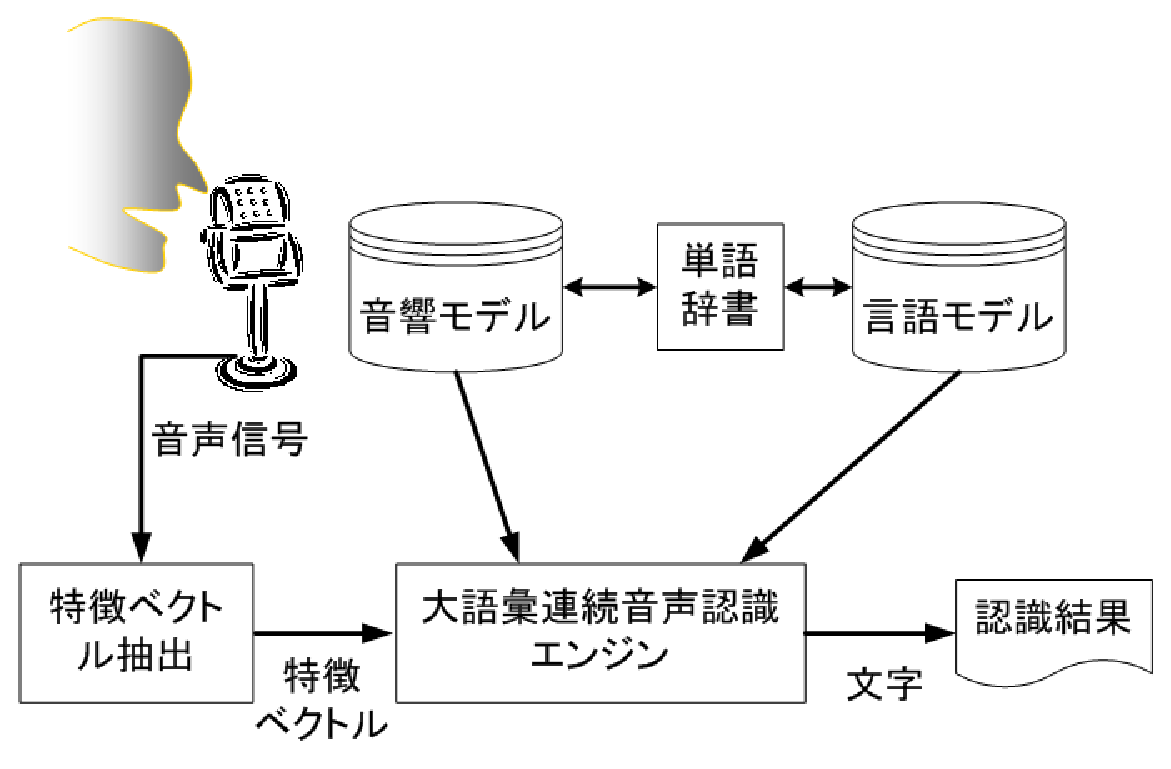
\includegraphics[width=14cm]{figures/recgsys.eps}
\caption{大語彙連続音声認識システム}     
\label{fig:bigrecgsys}
\end{center}
\end{figure}

表も作っておくと，図と表の目次ができる．
表~\ref{table:snr}は表の例である．

\begin{table}[htbp]
\caption{の度数分布}
\label{table:snr}
\begin{center}
\begin{tabular}{|c|r|r|r|} \hline
音素 & 平均フレーム長 & 分散 & 個数 \\ \hline
i & 6.814762 & 11.83095 & 132268 \\ \hline
u & 5.591616 & 10.67492 & 88505 \\ \hline
e & 7.98301 & 13.52340 & 85818 \\ \hline
o & 7.28116 & 14.32611 & 139195 \\ \hline
a: & 13.35346 & 13.50384 & 2054 \\ \hline
i: & 14.92981 & 20.96953 & 1724 \\ \hline
u: & 10.64128 & 17.49800 & 4831 \\ \hline
e: & 14.45515 & 15.58907 & 12688 \\ \hline
o: & 13.82564 & 19.01177 & 37657 \\ \hline
\end{tabular}
\end{center}
\end{table}

このスタイルの使い方について不備な点はあるが，まあ詳細はstyを読んで自分でがんがれ．


\section{本論文の構成}%\label{sec:structure}

本論文は\ref{chap:summary}章で構成される．

\ref{chap:jyoron}章では，いろいろなことを書いてある．

最後に\ref{chap:summary}章にて，本論文の成果をまとめ，今後の研究課題について述べる．
